\documentclass[12pt]{article}

% Packages
\usepackage[T1]{fontenc}
\usepackage[margin=1in]{geometry}
\usepackage{amsmath,amssymb}
\usepackage[numbers,sort&compress]{natbib}
\usepackage{graphicx}
\usepackage{booktabs}
\usepackage{xcolor}
\usepackage{hyperref}
\graphicspath{{../../../figures/}}

\title{Observational evidence for a meter or more of sea-level rise by 2100}
\author{Minchew et al.}
\date{}

\begin{document}
\maketitle

%% ================================================================
\begin{abstract}
Every centimeter of sea-level rise exposes roughly one million additional people to coastal flooding, yet the projections guiding adaptation planning rely on ice-sheet models whose outputs diverge below observed trends within years of initialization. We construct a data-driven baseline forecast by calibrating individual sea-level contributors with independent observations and validating against observed global mean sea level (GMSL). Our forecasts show that GMSL will likely rise 1.1~m (0.7--2.3 m, 90\% CI) by 2100 under current warming trends, exceeding the IPCC estimates by 40--70\% for the same warming and showing a 59\% probability of exceeding one meter. West Antarctic glacier dynamics, largely decoupled from 21st century emissions, accounts for 97\% of forecast uncertainty. The world is planning for roughly two-thirds of the sea-level rise the observations support.
\end{abstract}

%% ================================================================
\section*{Main text}

Rates of global mean sea-level rise have doubled twice since the beginning of the 20th century \citep{Frederikse2020} (Fig.~\ref{fig:observations} ***show rates on panel a***). The first doubling took about half a century and two-thirds of a degree of warming \citep{Rohde2020}. The second took half the time and slightly less warming. The rate will double again by 2080 if the current observed sea-level acceleration continues \citep{Hamlington2024}, and by roughly 2050 if it takes no more warming than the previous doublings. The 30-year gap between these two simple, data-driven predictions reflects the uncertainty that coastal adaptation must absorb. %Specifically, global mean sea level (GMSL) has risen 21~cm (19--23 cm, 90\% credible interval [CI]) since 1900 \citep{Frederikse2020}, with the rates increasing from 1.1~mm\,yr$^{-1}$ (0.8--1.3~mm\,yr$^{-1}$) averaged over 1900--1940 to 2.2~mm\,yr$^{-1}$ (1.2--3.2~mm\,yr$^{-1}$) in 1995 under $0.70 \pm 0.04\,^\circ$C of global mean surface temperature (GMST) warming, and then doubling again to 4.5~mm\,yr$^{-1}$ (3.5--5.5~mm\,yr$^{-1}$) by 2024 under an additional $0.63 \pm 0.07\,^\circ$C of warming \citep{Hamlington2024, Rohde2020}. 

%% ---- Figure 1: Observations ----
\begin{figure}[t]
\centering
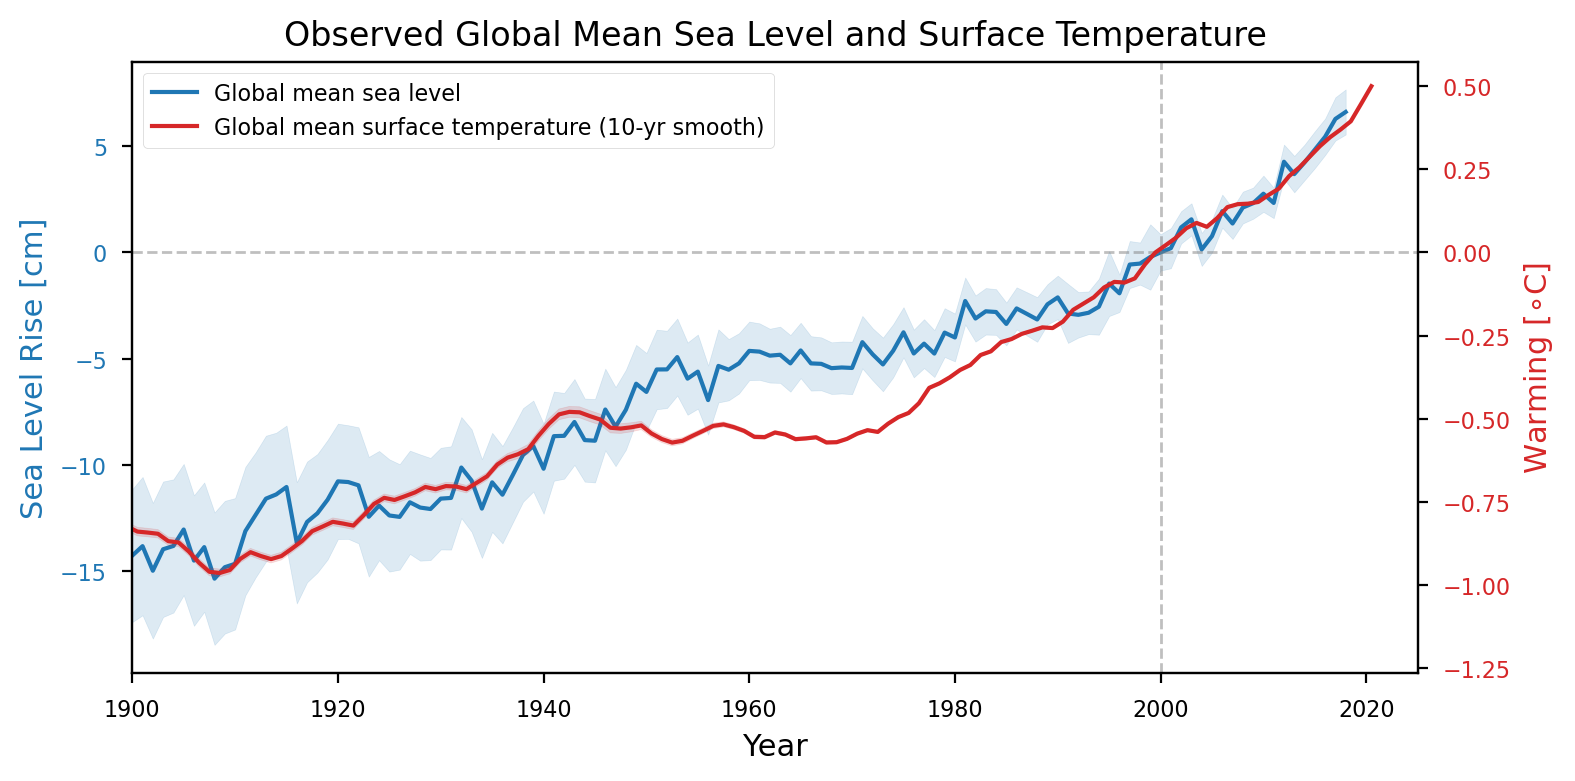
\includegraphics[width=\textwidth]{playing_w_figures_fig1_observations.png}\\[6pt]
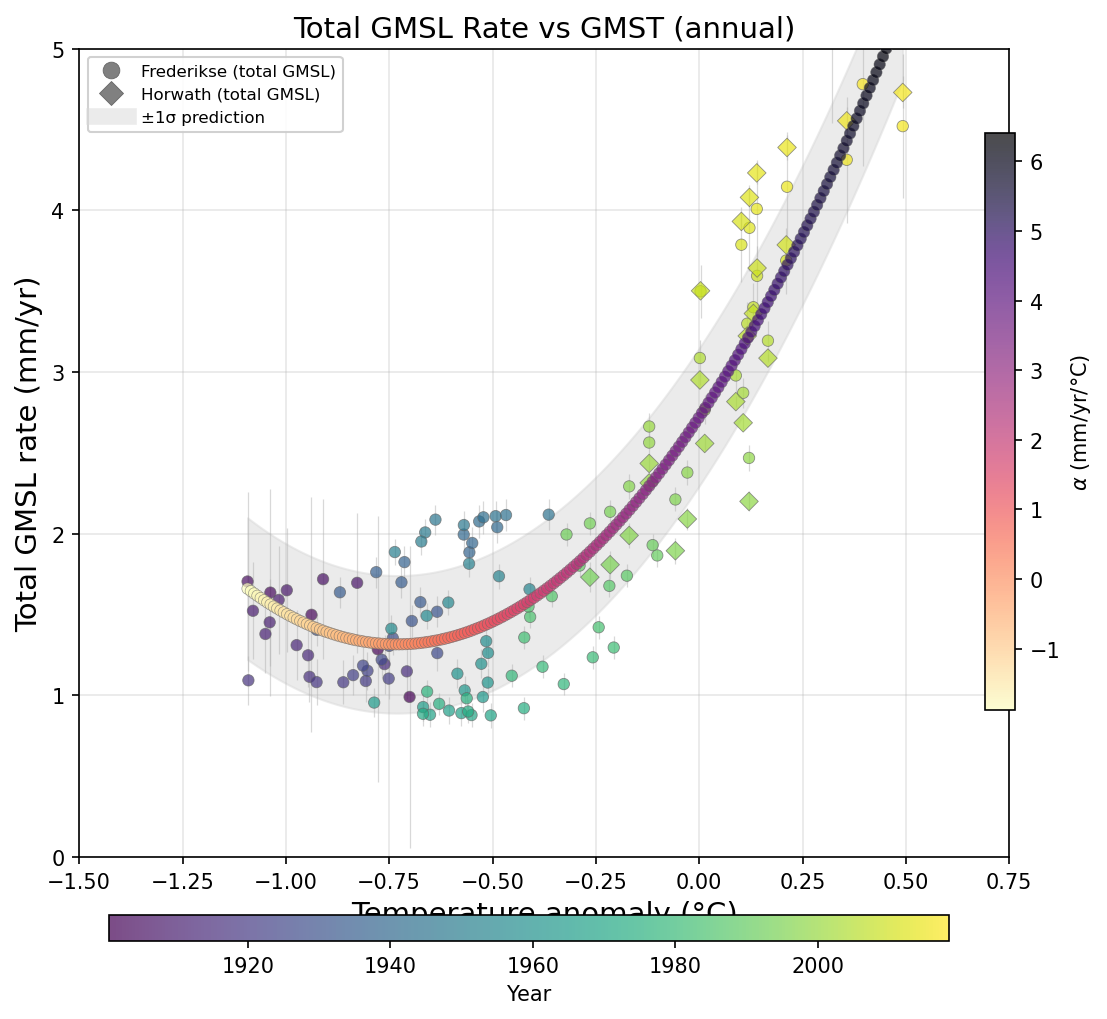
\includegraphics[width=0.48\textwidth]{total_gmsl_rate_vs_temperature_phase.png}%
\hfill%
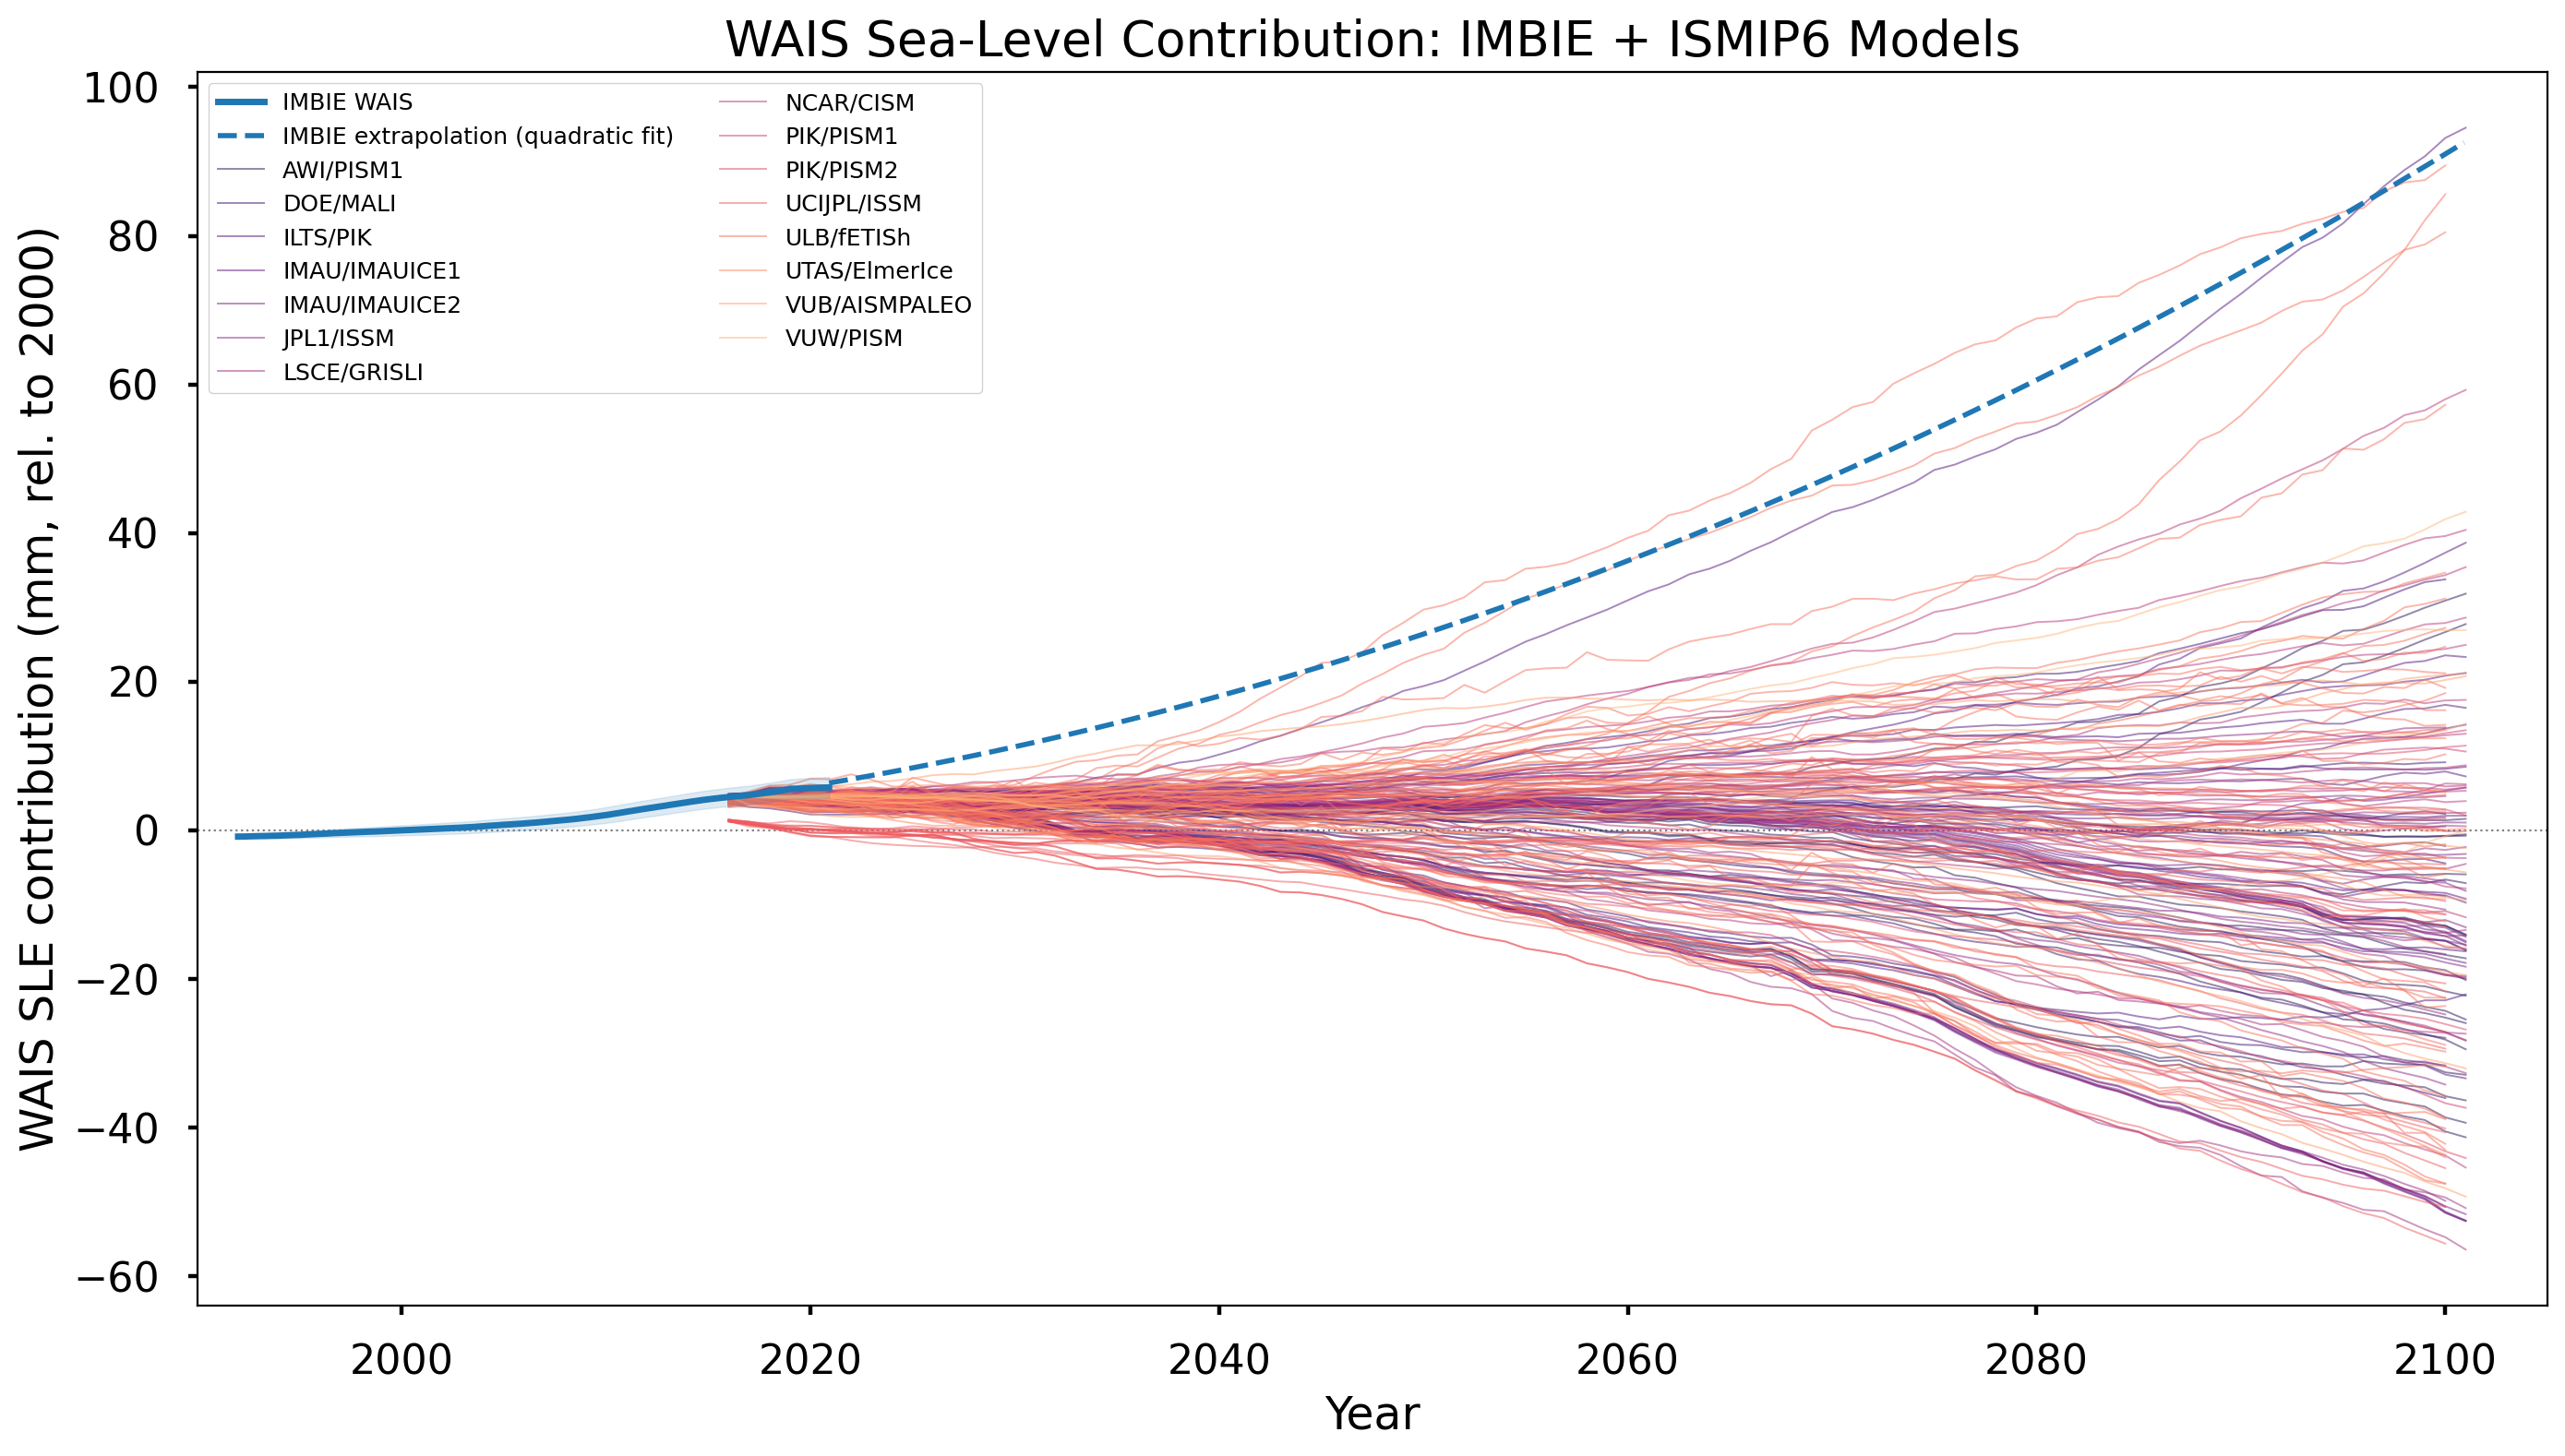
\includegraphics[width=0.48\textwidth]{wais_data_ipccar6_fig3_imbie_ismip6.png}
\caption{\textbf{Observed sea-level rise and the failure of process models.}
\textbf{(A)}~Observed GMSL (blue) and GMST (red, 10-year smooth) since 1900,
showing co-acceleration of warming and sea-level rise.  GMSL has risen
21~cm (19--23 cm, 90\% CI) since 1900, with the rate doubling from
1.1~mm\,yr$^{-1}$ (0.8--1.3~mm\,yr$^{-1}$) averaged over 1900--1940 to
2.2~mm\,yr$^{-1}$ (1.2--3.2~mm\,yr$^{-1}$) in 1995 under
$0.70 \pm 0.04\,^\circ$C of GMST warming, then doubling again to
4.5~mm\,yr$^{-1}$ (3.5--5.5~mm\,yr$^{-1}$) by 2024 under an additional
$0.63 \pm 0.07\,^\circ$C.
\textbf{(B)}~Total GMSL rate versus GMST anomaly, with the Bayesian
rate-and-state semi-empirical model (curve, colored by acceleration
$\alpha$; shading shows $\pm 1\sigma$ prediction interval).  The
nonlinear rate--temperature relationship explains the accelerating rate
doublings observed in~(A).
\textbf{(C)}~West Antarctic Ice Sheet: IMBIE satellite observations
(blue, 1992--2020) compared with ISMIP6 model projections used in AR6
(colored lines).  None of the 77 model runs reproduce the observed mass
loss; the models and observations diverge within years of initialization.}
\label{fig:observations}
\end{figure}

Every centimeter of rise exposes roughly one million additional people to coastal flooding \citep{Kulp2019}, approximately 90\% of whom live in low- and middle-income countries \citep{Jongman2012}. Without additional adaptation, annual flood damages are projected to reach US\$14--18~trillion per year for 0.9--1.1~m of rise \citep{Jevrejeva2018}. The cost of that adaptation is projected at US\$40--170~billion per year by mid-century \citep{Tiggeloven2020}, yet developing countries currently receive US\$21~billion per year in total adaptation finance across all sectors, not just coastal \citep{UNEP2023}, raising serious questions about the feasibility of coastal adaptation at the scale required and highlighting the value of reliable sea-level forecasts.

Most coastal adaptation planning relies on projections from the IPCC Sixth Assessment Report (AR6), which estimates 0.3--0.7~m of rise by 2100 relative to 1995--2014 \citep{Fox-Kemper2021, Hirschfeld2023}. These projections depend on process-based ice sheet models that diverge from satellite observations within years of initialization, with most producing ice sheets that gain mass under warming \citep{Aschwanden2021, Fricker2025} (Fig.~\ref{fig:observations}). As a result, observed GMSL trends already exceed AR6 medium-confidence projections under all emission scenarios \citep{Hamlington2022, Hamlington2024}. AR6 itself documents this: extrapolating the satellite-era trend and acceleration---which reflect the current warming trajectory, approximately SSP2-4.5---produces sea-level rise that matches or exceeds the process-based projections under SSP5-8.5, a scenario now widely regarded as implausible (AR6 Figure~9.27; \citep{Fox-Kemper2021,Hausfather2020}). The process models require an emissions pathway roughly twice the observed warming trajectory to reproduce the rates the ocean is already exhibiting. When model projections are inconsistent with observations under the realized forcing, those projections cannot serve as a reliable basis for planning.

Ice sheet models have known structural biases, including the absence of iceberg calving \citep{Fricker2025} and an assumed ice viscosity that is less sensitive to stress than satellite and laboratory observations indicate \citep{Millstein2022,Ranganathan2024,Fan2025}. The latter produces a 21--35\% underestimation of projected 21st century ice loss \citep{GetraerMorlighem2025, Martin2026}, while the absence of calving produces some unquantified error. More broadly, decades of forecasting research shows that models more complex than their calibration data can constrain produce worse out-of-sample predictions than simpler models \citep{Green2015, Makridakis2018}. Current ice sheet models have $\mathcal{O}(10^6)$ spatially distributed parameters (discretized basal friction and rheology fields), yet Hessian-based analyses show that surface velocity observations inform only a small fraction of these degrees of freedom, with the remainder determined by prior assumptions \citep{Isaac2015, Petra2014}.

We construct a data-driven, hierarchical baseline forecast that inverts this ratio by focusing on different sea-level contributors, each with minimal physical parameters constrained by independent observational records spanning decades. Observed total sea level (GMSL) is a diagnostic sum, and we show budget closure within 12\% with our approach. Our framework makes the assumptions explicit and transparent with quantified uncertainties, providing a benchmark against more complex models can be tested. Unless otherwise noted, all sea-level values in the main text are 21st-century contributions referenced to the year 2000, while values in the abstract are relative to pre-industrial for consistency with existing projections and literature. Throughout, we label emission scenarios by their approximate end-of-century global mean surface temperature: 2$\,^\circ$C (SSP1-2.6), 3$\,^\circ$C (SSP2-4.5), 4$\,^\circ$C (SSP3-7.0), and 5$\,^\circ$C (SSP5-8.5).

\subsection*{Data-driven framework}

Our framework draws on two established lines of data-driven forecasting. The simplest requires no model at all. A quadratic fit to the satellite altimetry record (1993--present) extrapolated to 2100 \citep{Hamlington2022, Hamlington2024} yields a median of 66~cm (41--91 cm) of 21st-century rise, already exceeding IPCC medians for a 3$^\circ$C trajectory (SSP2-4.5; 56~cm) and approaching a 4$^\circ$C trajectory (SSP3-7.0; 68~cm). The 32-year satellite record robustly constrains the current rate and acceleration of GMSL, giving the quadratic extrapolation predictive skill over the next one to two decades (roughly half the calibration window) before changes in forcing or ice dynamics could alter the trajectory. Beyond that horizon, the quadratic still establishes a scenario-independent benchmark that any credible forecast must meet or explain. 

Semi-empirical models relate the rate of GMSL rise to changes in global mean surface temperature (GMST). Under current warming trends, Rahmstrof (2007) \citep{Rahmstorf2007} predicts 0.67~m (0.63--0.71 m) of 21st-century rise, closely matching the extrapolation of modern observations \citep{Hamlington2024}, while the updated model \citep{Vermeer2009}, which adds a rate-of-warming term, predicts 0.96~m (0.80--1.12 m). Although physically motivated by the fit to sensitivities rather than rates, semi-empirical models were assessed as \emph{low confidence} by IPCC AR5 because they do not resolve individual contributing processes and because extrapolation beyond the calibration period assumes a stationary temperature--sea-level relationship \citep{Church2013}. This reasoning contradicts the decision of AR5 and AR6 to favor process models that omit key physics such as calving, use untested parameterizations of ocean-induced melting, are initialized with static data fields and then run forward in time, and were never validated against observed GMSL, the very quantity they attempt to predict (cf.\ AR6 Figure~9.27 in \citep{Fox-Kemper2021}). In short, the IPCC set aside simple, data-driven models consistent with observations in favor of complex process models that fail to reproduce them. %A recent evaluation of IPCC GMSL projections against the satellite record found that apparent agreement arose from compensating component-level errors \citep{Tornqvist2025}. 

%Our framework extends existing data-driven approaches by decomposing the aggregate GMSL signal into its components, and fits the most reduced physically justified models we could support with the scholarly literature and validate with data. A Bayesian framework provides structured uncertainty quantification for the fitted sensitivities, allowing uncertainty attribution in the predicted values. Where there are not enough data, such as for terrestrial water storage and the surface mass balance of ice sheets, we fall back to established models or, in the case of West Antarctic Ice Sheet (WAIS), a scenario-scheme that attempts to capture much of the known knowledge gaps. It is important to note that the scenario approach for WAIS is not a robust uncertainty, but rather a representation of the many ideas and results currently represented in the scholarly literature. Robust uncertainty quantification for WAIS is, arguably, not possible at this time due to a severe dearth of data. 

%% ================================================================
\subsection*{Component decomposition}

We decompose global mean sea level into seven components: ocean thermal expansion (thermosteric), mountain glaciers, Greenland surface mass balance (SMB), Greenland ice discharge, West Antarctic Ice Sheet (WAIS), East Antarctic Ice Sheet (EAIS), and the Antarctic Peninsula. Each is calibrated against independent observational datasets spanning 24--71 years of direct measurements (Table~S1, Materials and Methods).

\paragraph{Ocean thermal expansion.} The thermosteric component---the largest single contributor to observed sea level rise---uses NOAA in situ observations \citep{Levitus2012} for the hindcast (0--700\,m from 1955, 0--2000\,m from 2005), supplemented by literature-derived corrections for deeper layers \citep{Purkey2010, Cheng2017}, and IPCC AR6 projections \citep{Fox-Kemper2021} for the future. The IPCC thermosteric projections are based on a two-layer energy balance model \citep{Geoffroy2013} constrained by observed global temperature and ocean heat content---the same physics our original custom model employed, making independent refitting unnecessary. We include a 14\% structural uncertainty on the NOAA observations reflecting the documented low bias from interpolation of sparse hydrographic profiles \citep{Li2022}.

\paragraph{Glaciers.} Mountain glacier mass loss is modeled as a rate--temperature relationship calibrated against the GlaMBIE global consensus \citep[2000--2024;][]{GlaMBIE2024}, the first globally complete, observation-only glacier mass-balance record. The fitted linear sensitivity is $b_{\mathrm{gl}} = 0.77$~mm\,yr$^{-1}$\,$^\circ$C$^{-1}$. This is approximately six times the value embedded in IPCC AR6 median projections ($\sim$0.13~mm\,yr$^{-1}$\,$^\circ$C$^{-1}$) and 1.5--2$\times$ the effective sensitivity of the PyGEM process model \citep{Rounce2023}. The IPCC rate structure is inverted relative to observations: IPCC attributes most glacier mass loss to a temperature-independent committed response, whereas the data show mass loss driven primarily by ongoing warming. A hard ceiling at the total glacier ice volume ($\sim$0.32~m sea level equivalent; Farinotti et~al.~\cite{Farinotti2019}) bounds cumulative loss.

\paragraph{Greenland.} We treat Greenland SMB and ice discharge separately. SMB observations from RACMO \citep{Mouginot2019, Noel2018} are used directly for the hindcast; forecasts scale with temperature using sensitivities from regional climate model intercomparisons \citep{Fettweis2020, Noel2021}. The choice of regional climate model (RACMO-only vs.\ a three-model average including MAR and HIRHAM) does not materially affect the hindcast (4\% difference; Supplementary Material). RACMO sits at the conservative end of the RCM range: all models systematically underestimate ablation-zone melt relative to in situ observations \citep{Fettweis2020}, and RACMO's bare-ice albedo remains too high despite partial MODIS assimilation \citep{Alexander2022, Noel2019}. Under strong warming, the inter-RCM spread becomes a factor of two in projected SMB \citep{Glaude2024}; this structural uncertainty is captured in our forecast priors but not in the hindcast, where RACMO-derived SMB should be regarded as a conservative estimate of Greenland surface mass loss.

Greenland discharge is modeled as a time-delay response to subsurface ocean warming:
\begin{equation}
	\Delta H_{\mathrm{dyn}}(t) = \gamma \int_{t_0}^{t} T_{\mathrm{ocean}}(t' - \delta)\, dt' + r_0\,(t - \bar{t}),
	\label{eq:greenland_dyn}
\end{equation}
where $\gamma$ is the discharge sensitivity to ocean temperature, $\delta$ is the time delay between ocean warming and the ice sheet response, and $r_0$ is a secular drift from post--Little Ice Age adjustment. Cross-correlation of EN4 subsurface ocean temperature \citep{Good2013} against the Mouginot et~al.~\citep{Mouginot2019} discharge record identifies a peak at $\delta = 6$~yr ($r = 0.84$); BIC model selection gives $\delta = 5$~yr ($R^2 = 0.995$). All three parameters can be independently derived from glacier dynamics (Supplementary Material): the fitted coupling $\gamma = 0.365$~mm\,yr$^{-1}$\,$^\circ$C$^{-1}$ agrees with bottom-up physical estimates (0.36~mm\,yr$^{-1}$\,$^\circ$C$^{-1}$) to within 2\%, providing independent validation that the model captures the governing physics. The Mankoff et~al.~\citep{Mankoff2021} discharge record (1986--2023) and NOAA Arctic Report Card estimates, withheld from calibration, fall within the 90\% credible interval.

\paragraph{West Antarctica.} WAIS is the dominant source of forecast uncertainty. The ice sheet contains $\sim$3.3~m of sea level equivalent on retrograde beds susceptible to marine ice sheet instability (MISI; Joughin et~al.~\cite{Joughin2014}), and ocean thermal forcing sufficient to drive retreat is committed regardless of emissions pathway \citep{Naughten2023}. We construct a scenario-mixture framework combining three outcomes---continued present-day rates, MISI-driven acceleration, and MISI with additional cliff instability---with physically motivated within-scenario skewness \citep{Robel2019} and a rheology correction reflecting the $n = 3 \to 4$ bias documented in all current ice sheet models \citep{Martin2026, GetraerMorlighem2025}. The resulting distribution is wider than the structured expert judgment of Bamber et~al.~\citep{Bamber2019} (which predates the rheology correction) but in broad agreement, providing independent methodological corroboration.

%% ================================================================
\subsection*{Budget closure and validation}

Each component is calibrated independently; the total sea level is a diagnostic sum, not a calibration target. Over the satellite era (1993--2020), the component sum tracks NASA altimetry with a residual rate trend of 0.37~mm\,yr$^{-1}$. A variance-weighted attribution distributes this residual across components in proportion to their uncertainties. The thermosteric component absorbs the largest share (57\%), consistent with the known low bias in the NOAA product \citep{Li2022, Cheng2017}. Terrestrial water storage absorbs 23\%, reflecting poorly characterized structural uncertainty in groundwater and reservoir reconstructions. All ice-related components---glaciers, Greenland, WAIS---are within 1.5 standard deviations of their independent estimates. The framework closes the observed budget without requiring any component to depart from what the observations support.

%% ================================================================
\subsection*{Forecasts}

We focus on SSP1-2.6 through SSP3-7.0, the pathways most consistent with current policies and stated pledges; SSP5-8.5 is now widely regarded as implausible under implemented and pledged policies \citep{Hausfather2020} and is reported only for comparability with prior literature.

Under SSP1-2.6 (aggressive emissions cuts consistent with the Paris Agreement 2$\,^\circ$C target; the AR6 temperature trajectory includes mid-century overshoot, which is relevant because ice loss is largely irreversible on policy timescales), the blended forecast projects 75~cm of 21st-century sea-level rise by 2100 [5th--95th percentile: 42--183~cm], 70\% above the IPCC AR6 medium-confidence estimate of 44~cm. Under SSP2-4.5 (intermediate emissions), the median is 86~cm [53--196~cm], 53\% above IPCC's 56~cm. Under SSP3-7.0, the median reaches 98~cm [64--207~cm]. For reference, SSP5-8.5 yields a median of 107~cm [73--215~cm].

Relative to pre-industrial levels (adding $\sim$0.19~m of observed rise through 2000), these forecasts correspond to medians of 0.94--1.17~m across policy-relevant pathways. The probability of exceeding 1~m relative to pre-industrial by 2100 is 42\% under SSP1-2.6, 58\% under SSP2-4.5, and 78\% under SSP3-7.0. Averaged across these pathways, the probability is 59\%, largely insensitive to the relative weighting of scenarios.

The within-scenario 90\% uncertainty range (143~cm for SSP2-4.5) is six times larger than the spread across scenario medians (23~cm from SSP1-2.6 to SSP3-7.0). A variance decomposition (law of total variance across policy SSPs) attributes 97\% of total forecast variance to within-scenario uncertainty---predominantly WAIS---and 3\% to between-scenario differences. This reflects the dominance of WAIS uncertainty, which is largely independent of the emission pathway: ocean thermal forcing sufficient to sustain WAIS retreat is committed regardless of emissions \citep{Naughten2023}. The scenario spread arises from the temperature-sensitive components---primarily glaciers and the Greenland ice sheet---whose observationally calibrated sensitivities substantially exceed those in current consensus projections. The discrepancy with IPCC is accordingly largest under low warming (1.7$\times$ for SSP1-2.6) and narrows toward high warming (1.4$\times$ for SSP3-7.0), because the glacier sensitivity dominates at moderate warming but the finite glacier ice reservoir caps cumulative loss under strong warming. The thermosteric component, adopted directly from IPCC AR6, contributes no additional excess.

The forecast blends two independent constraints: a satellite-era quadratic extrapolation (scenario-independent; median 63~cm of 21st-century rise) that anchors the near-term trajectory, and the component-level model sum that captures scenario-dependent physics over longer horizons. The blending is performed in rate space via a sigmoid transition centered at 2035, ensuring continuity in both level and rate at the forecast origin while allowing the component models to govern the long-term response. The satellite-era quadratic alone---requiring no model and no emissions scenario---already exceeds IPCC medians under SSP1-2.6 and SSP2-4.5.

%% ---- Figure 1: Total GMSL forecast ----
%\begin{figure}[t]
%\centering
%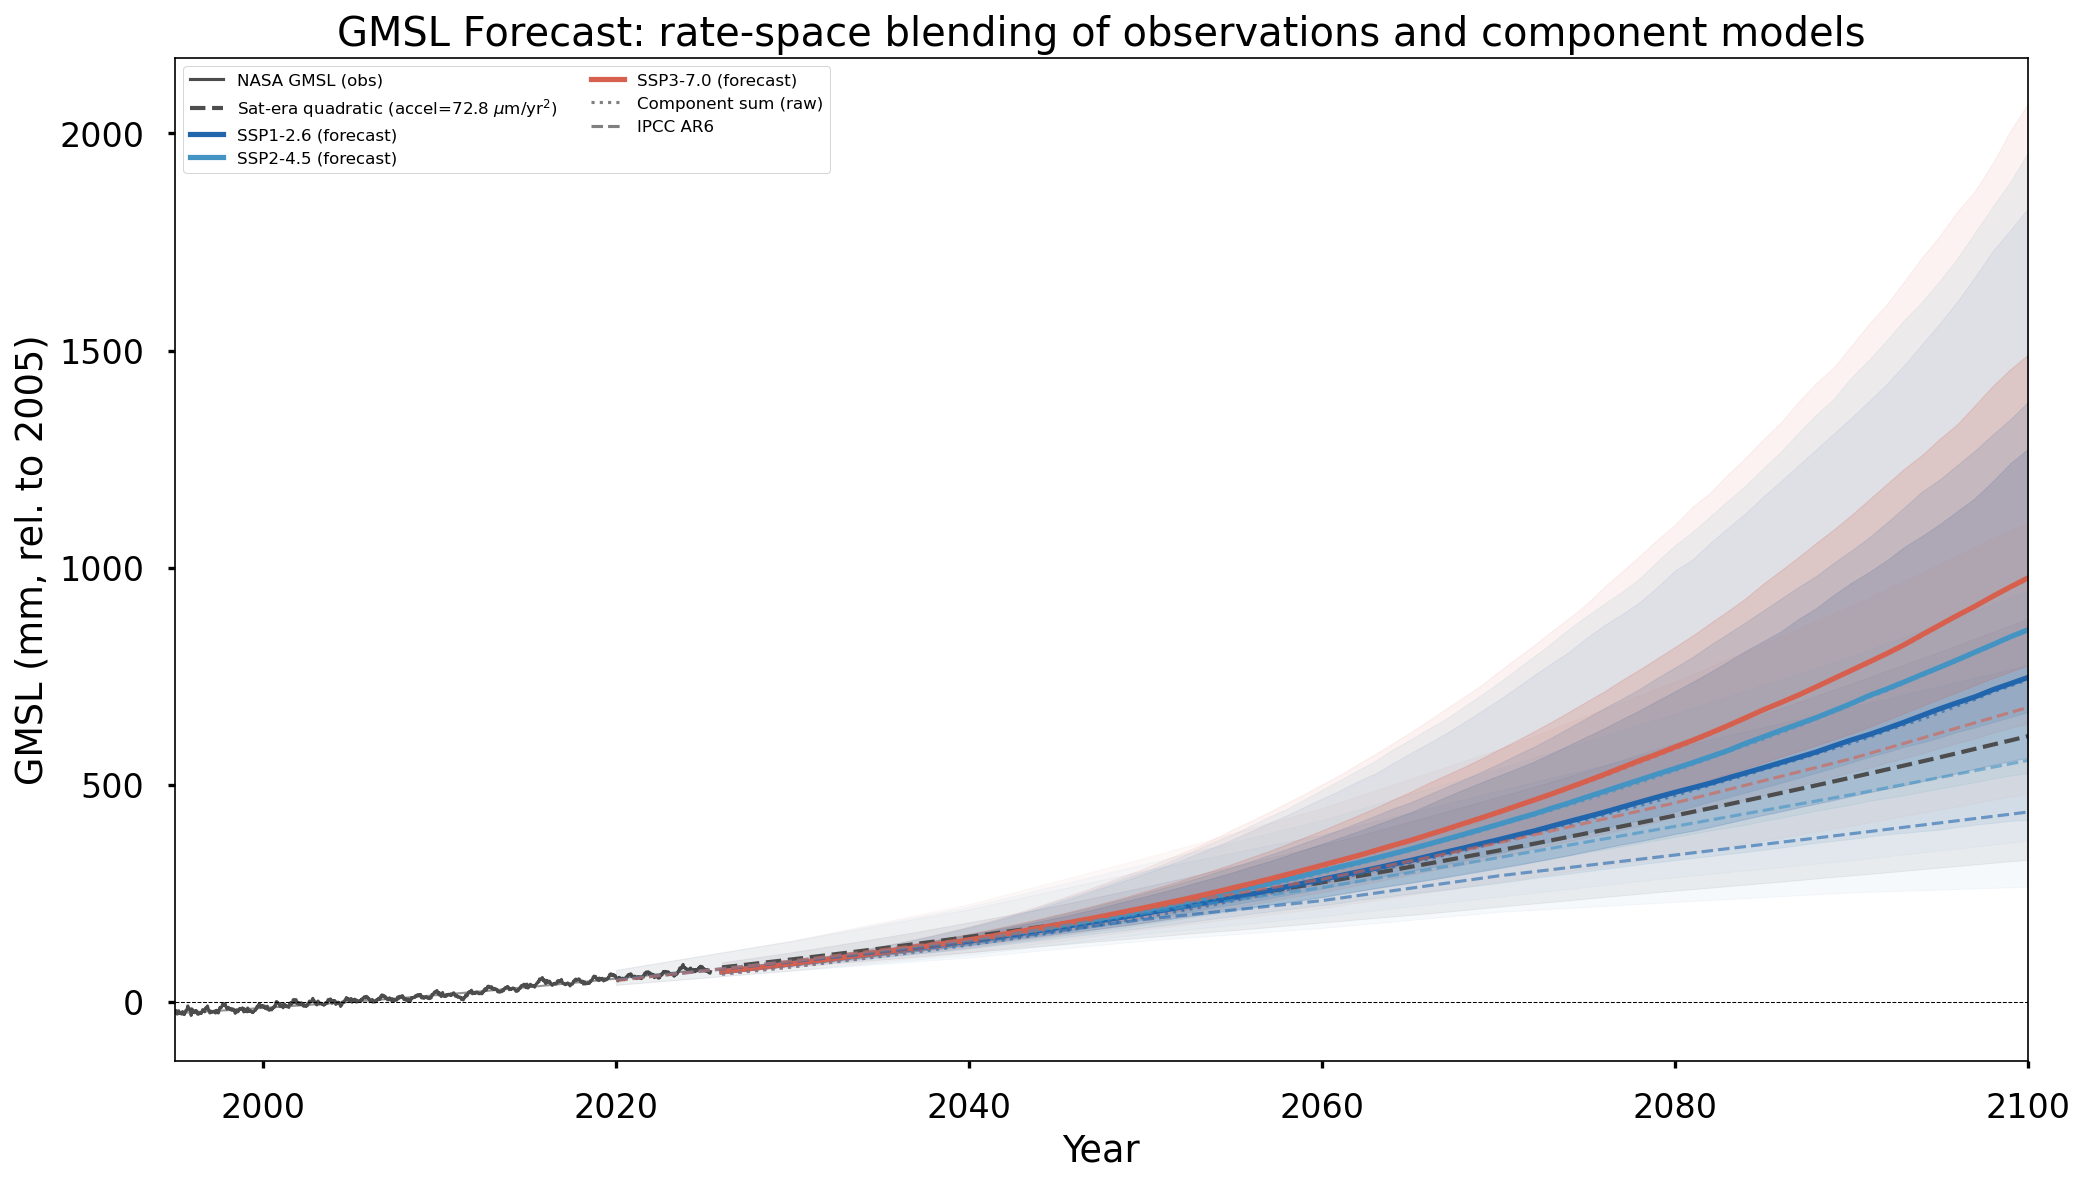
\includegraphics[width=\textwidth]{component_forecast_total.png}
%\caption{\textbf{Global mean sea level forecast.}
%NASA satellite altimetry observations (black, 1993--2025) and blended
%forecasts under SSP1-2.6 (blue), SSP2-4.5 (teal), and SSP3-7.0 (orange),
%with shading showing the 66\% (dark) and 90\% (light) credible intervals.
%The satellite-era quadratic extrapolation (grey dashed) anchors the
%near-term trajectory and is blended into the component-sum physics via a
%sigmoid transition centered at 2035.  IPCC AR6 medium-confidence medians
%(dashed colored lines) and the raw component sum (dotted) are shown for
%comparison.  The quadratic extrapolation alone (63~cm median, grey) already
%exceeds IPCC medians under SSP1-2.6 and SSP2-4.5.  All values are relative
%to the 2005 baseline.}
%\label{fig:forecast_total}
%\end{figure}

%% ---- Figure 2: Per-component breakdown ----
%\begin{figure}[t]
%\centering
%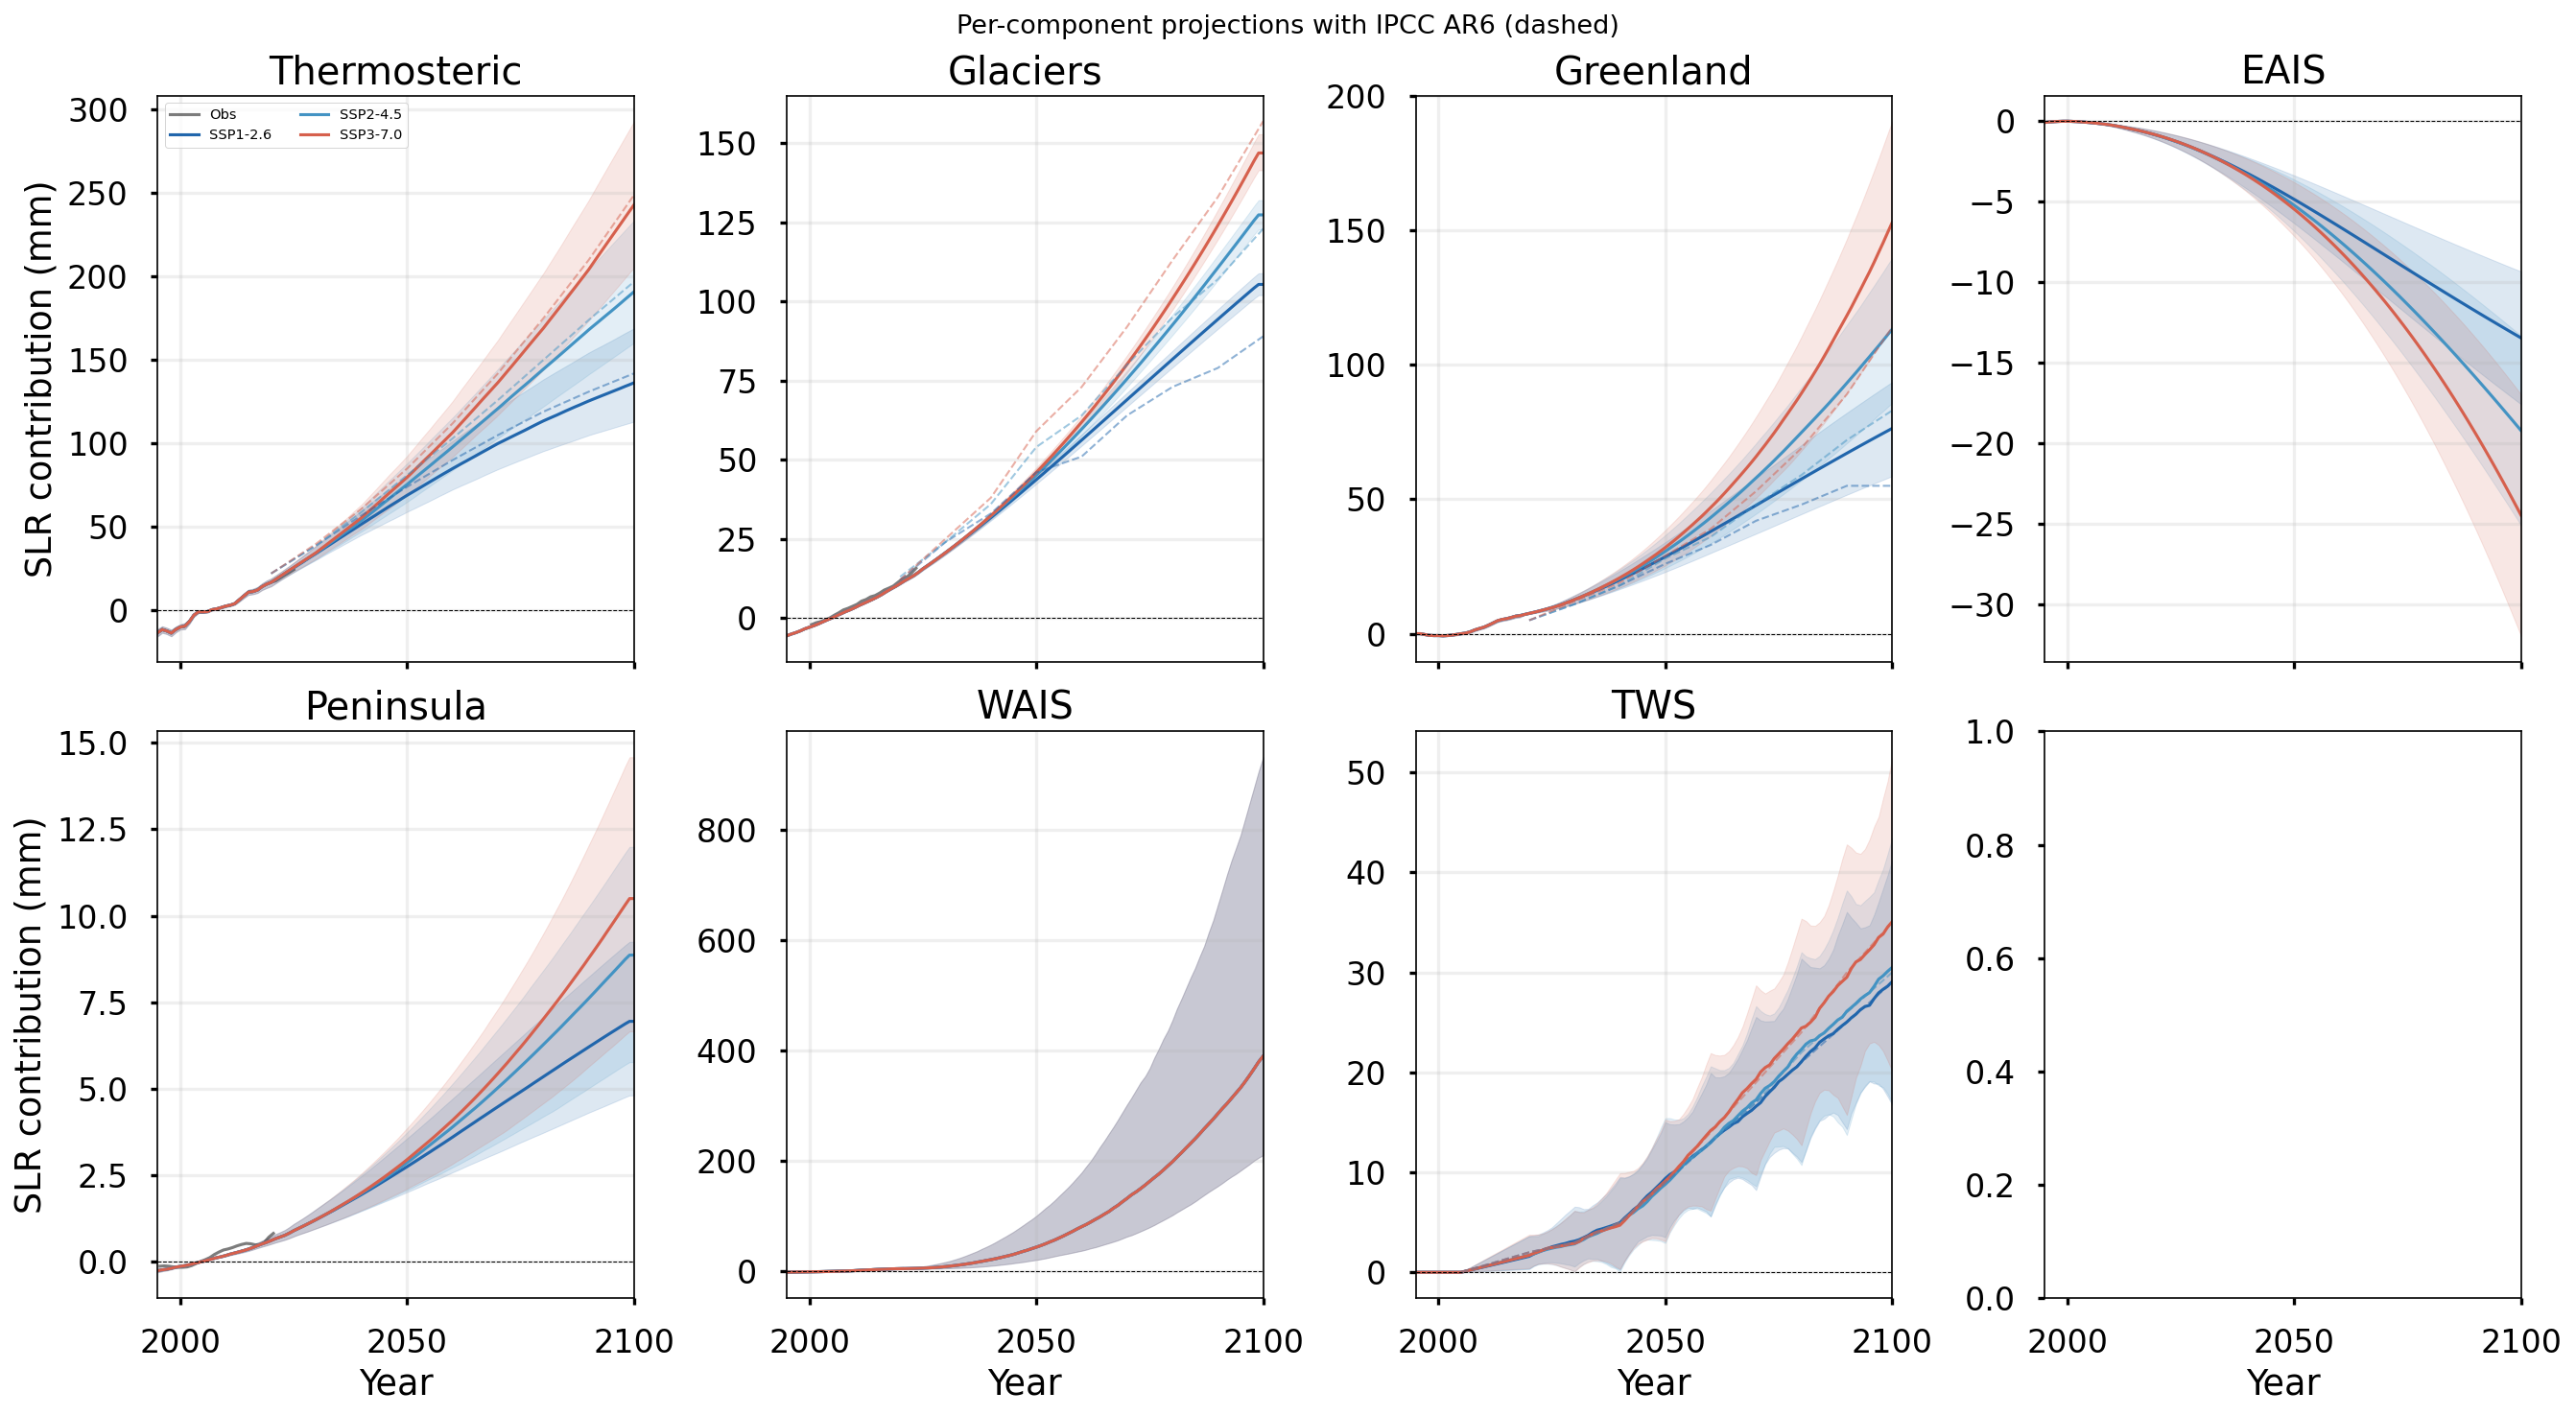
\includegraphics[width=\textwidth]{component_forecast_per_component.png}
%\caption{\textbf{Per-component projections compared with IPCC AR6.}
%Individual sea-level contributors (panels) showing our median projections
%(solid) and 66\% credible intervals (shading) for SSP1-2.6 (blue),
%SSP2-4.5 (teal), and SSP3-7.0 (orange), with IPCC AR6 component medians
%(dashed) overlaid.  Observations (grey) anchor each component.  The
%discrepancy with IPCC originates primarily from glaciers (sensitivity
%six times higher than IPCC's effective value) and WAIS (wider uncertainty
%from the A4 deep-uncertainty framework including rheology correction).
%The thermosteric component is adopted from IPCC and contributes no
%additional excess.  EAIS contributes negative SLR (mass gain from
%increased snowfall under warming).  All values in mm relative to the 2005
%baseline.}
%\label{fig:per_component}
%\end{figure}

%% ---- Figure 3: Ice sheet dynamics ----
% TODO: Generate publication figure combining Greenland discharge + WAIS
%       ISMIP6 comparison.  Placeholder panels shown below.
%\begin{figure}[t]
%\centering
%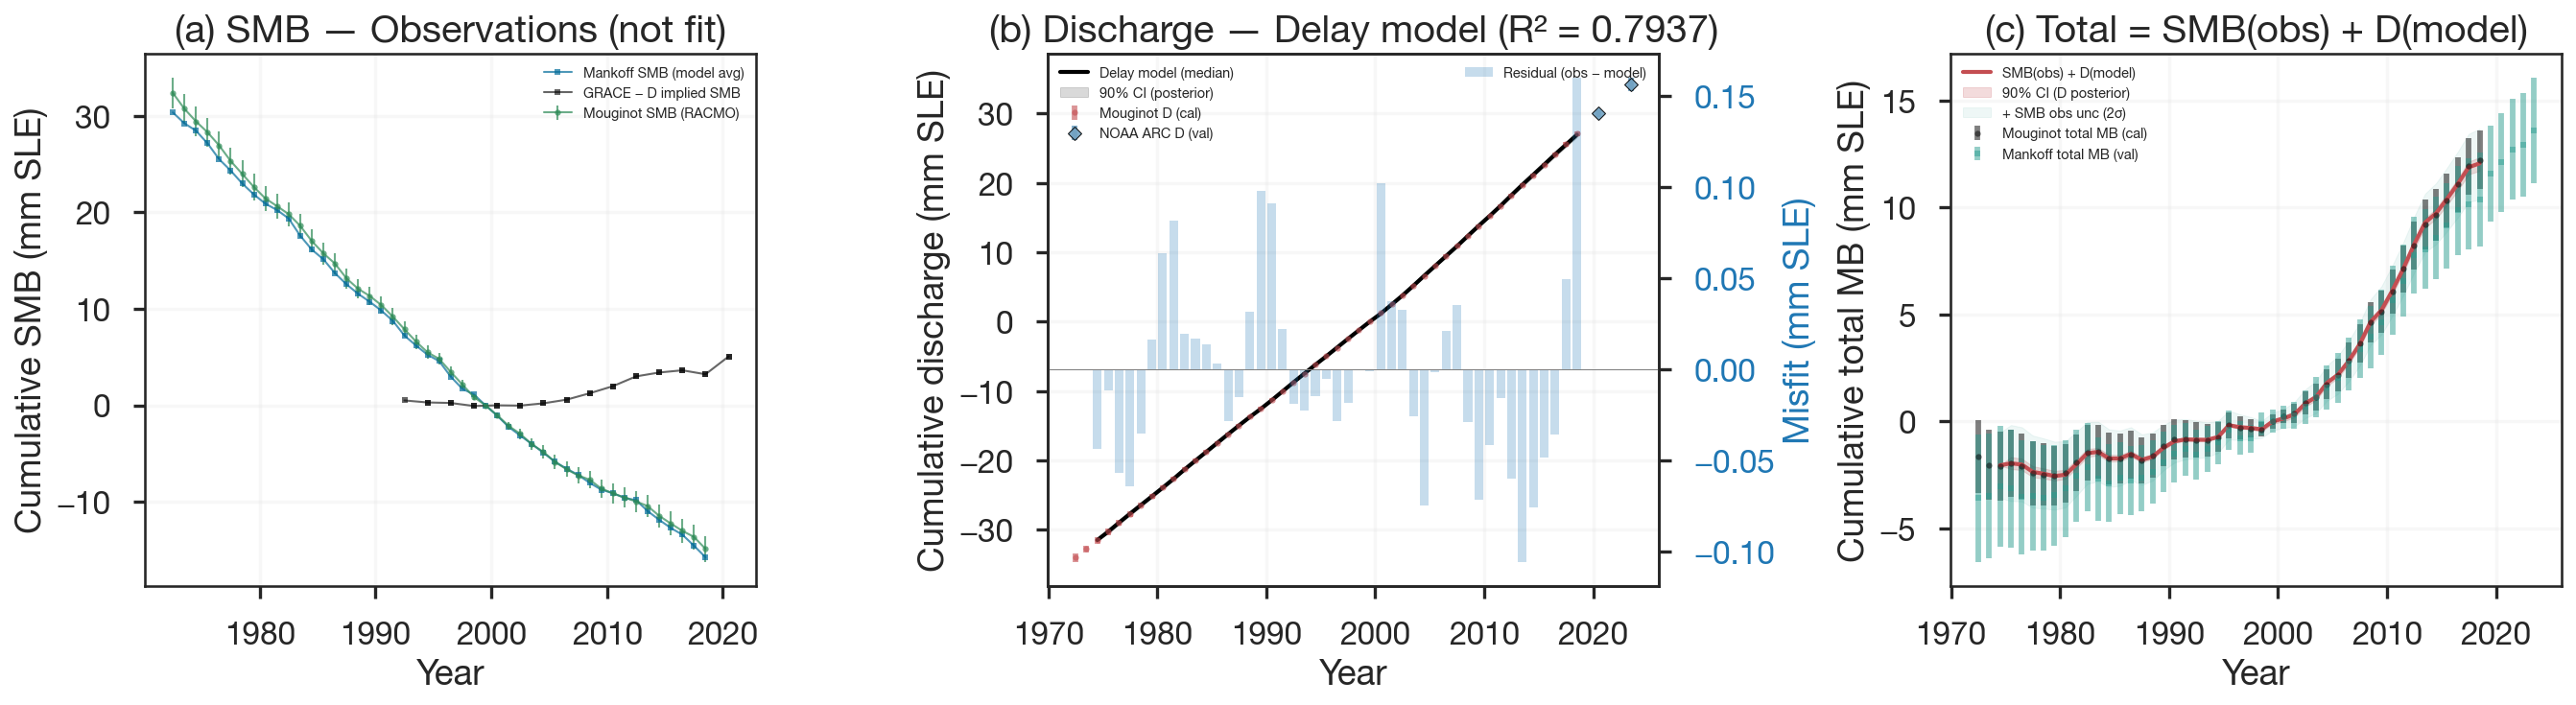
\includegraphics[width=0.48\textwidth]{component_greenland_smb_d_fit.png}%
%\hfill%
%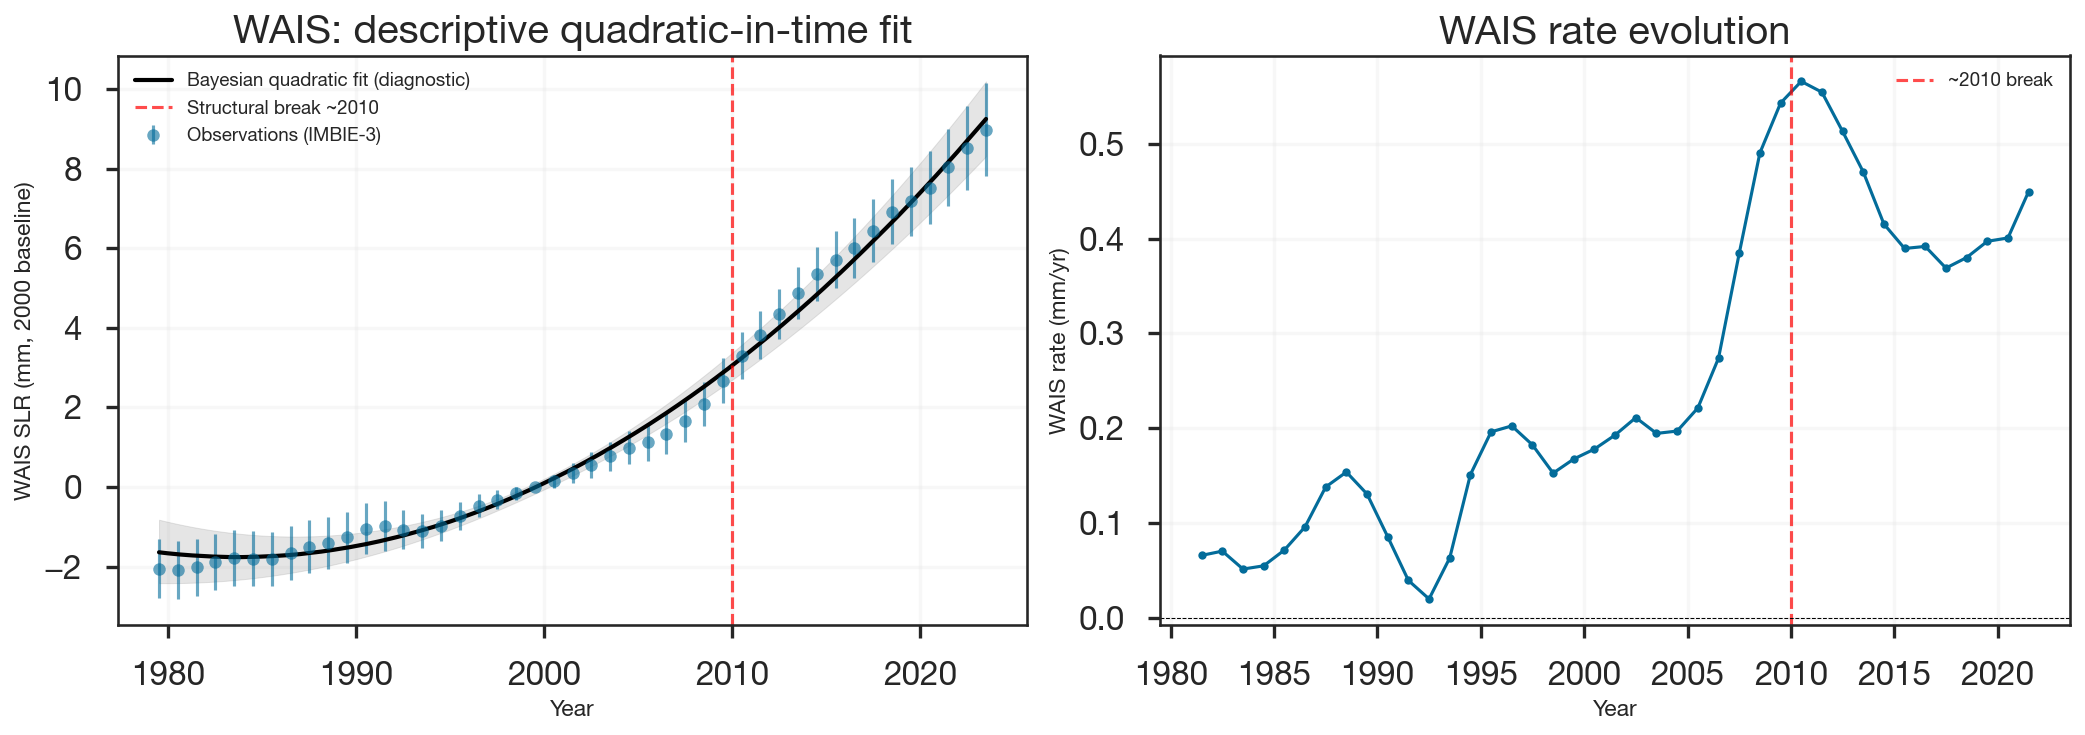
\includegraphics[width=0.48\textwidth]{component_wais_observations.png}
%\caption{\textbf{Ice sheet dynamics: Greenland discharge model and WAIS
%model--observation divergence.}
%\textbf{(A)}~Greenland ice discharge modeled as a time-delay response to
%subsurface ocean warming (Eq.~\ref{eq:greenland_dyn}).  The fitted model
%($\delta = 5$~yr, $R^2 = 0.995$) captures 46 years of observed discharge
%variability (Mouginot et~al., 1972--2018; filled circles).  The Mankoff
%et~al.\ (1986--2023) record, withheld from calibration, falls within the
%90\% credible interval (grey shading), providing independent validation.
%All three model parameters ($\gamma$, $\delta$, $r_0$) agree with
%independent physical estimates to within 2--40\% (Supplementary Material).
%\textbf{(B)}~West Antarctic Ice Sheet: IMBIE satellite observations
%(1992--2020; black) showing 5.0~mm of cumulative sea-level contribution,
%compared with 77 ISMIP6 model trajectories (colored lines, derived as
%total AIS minus EAIS minus Peninsula).  At 2020, 0 of 77 ISMIP6 runs
%reproduce the observed mass loss (median model value: 0.8~mm vs.\
%observed 5.0~mm); 12\% of runs show WAIS gaining mass.  The divergence
%reflects known structural biases: absence of calving, incorrect ice
%rheology ($n = 3$ vs.\ observed $n \approx 4$; Martin et~al.~\cite{Martin2026}),
%and missing subglacial hydrology.}
%\label{fig:ice_sheets}
%\end{figure}

%% ---- Figure 4: Uncertainty structure ----
% TODO: Generate publication figure combining exceedance curves +
%       variance decomposition.  Placeholder below.
%\begin{figure}[t]
%\centering
%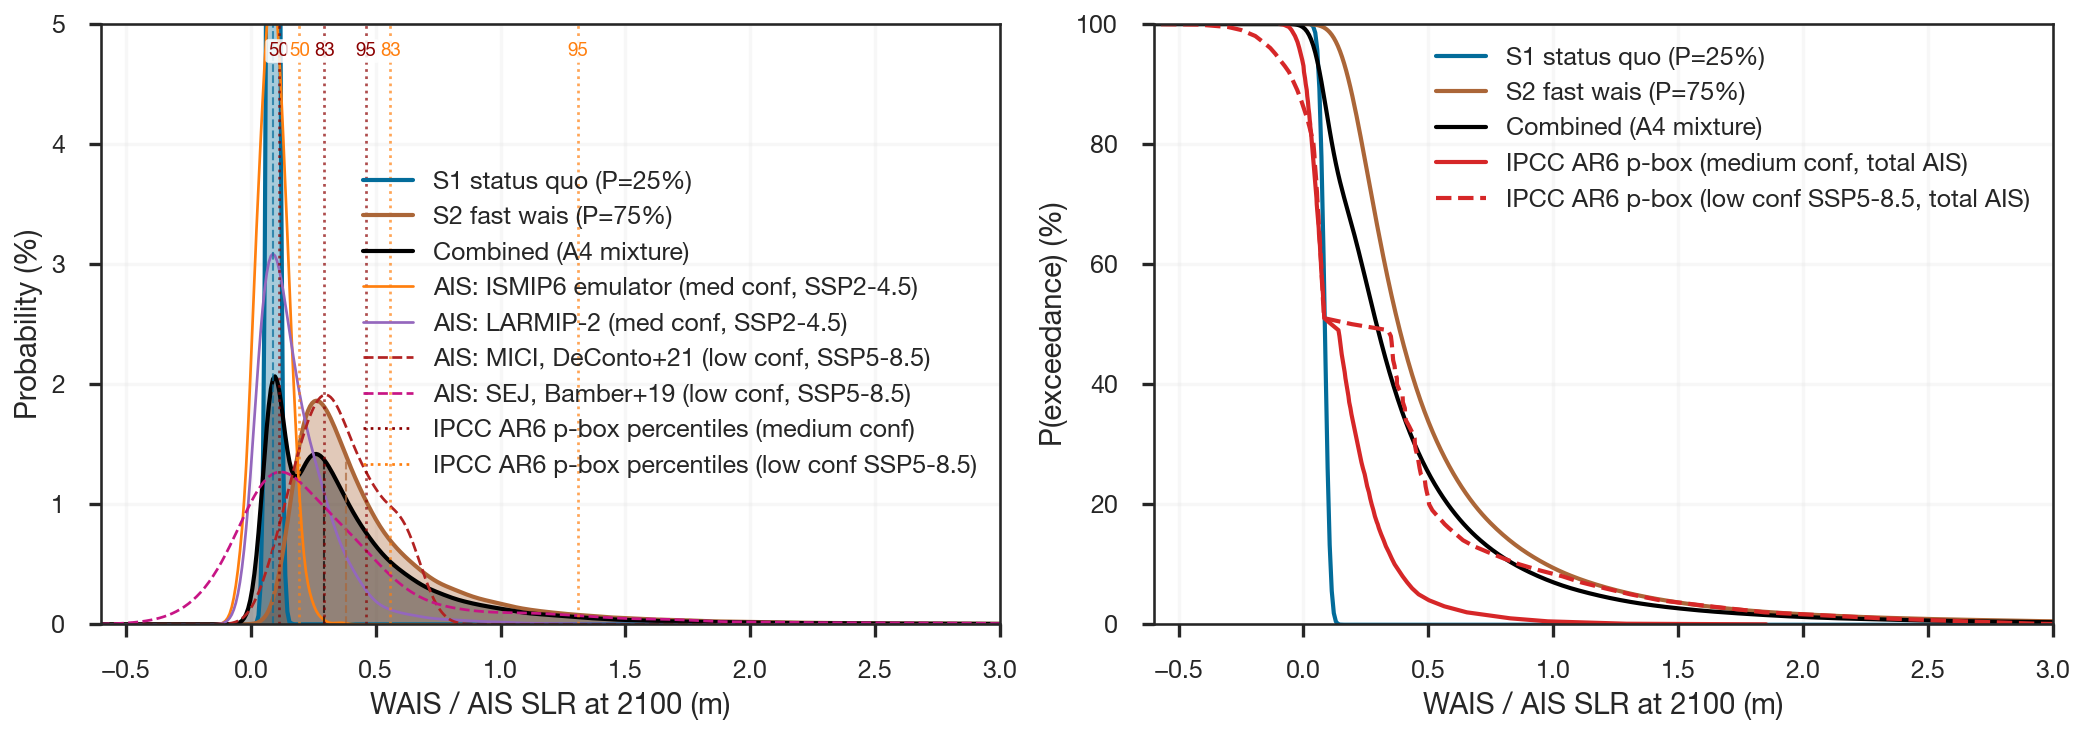
\includegraphics[width=0.48\textwidth]{component_wais_pdf_exceedance_ipcc.png}%
%\hfill%
%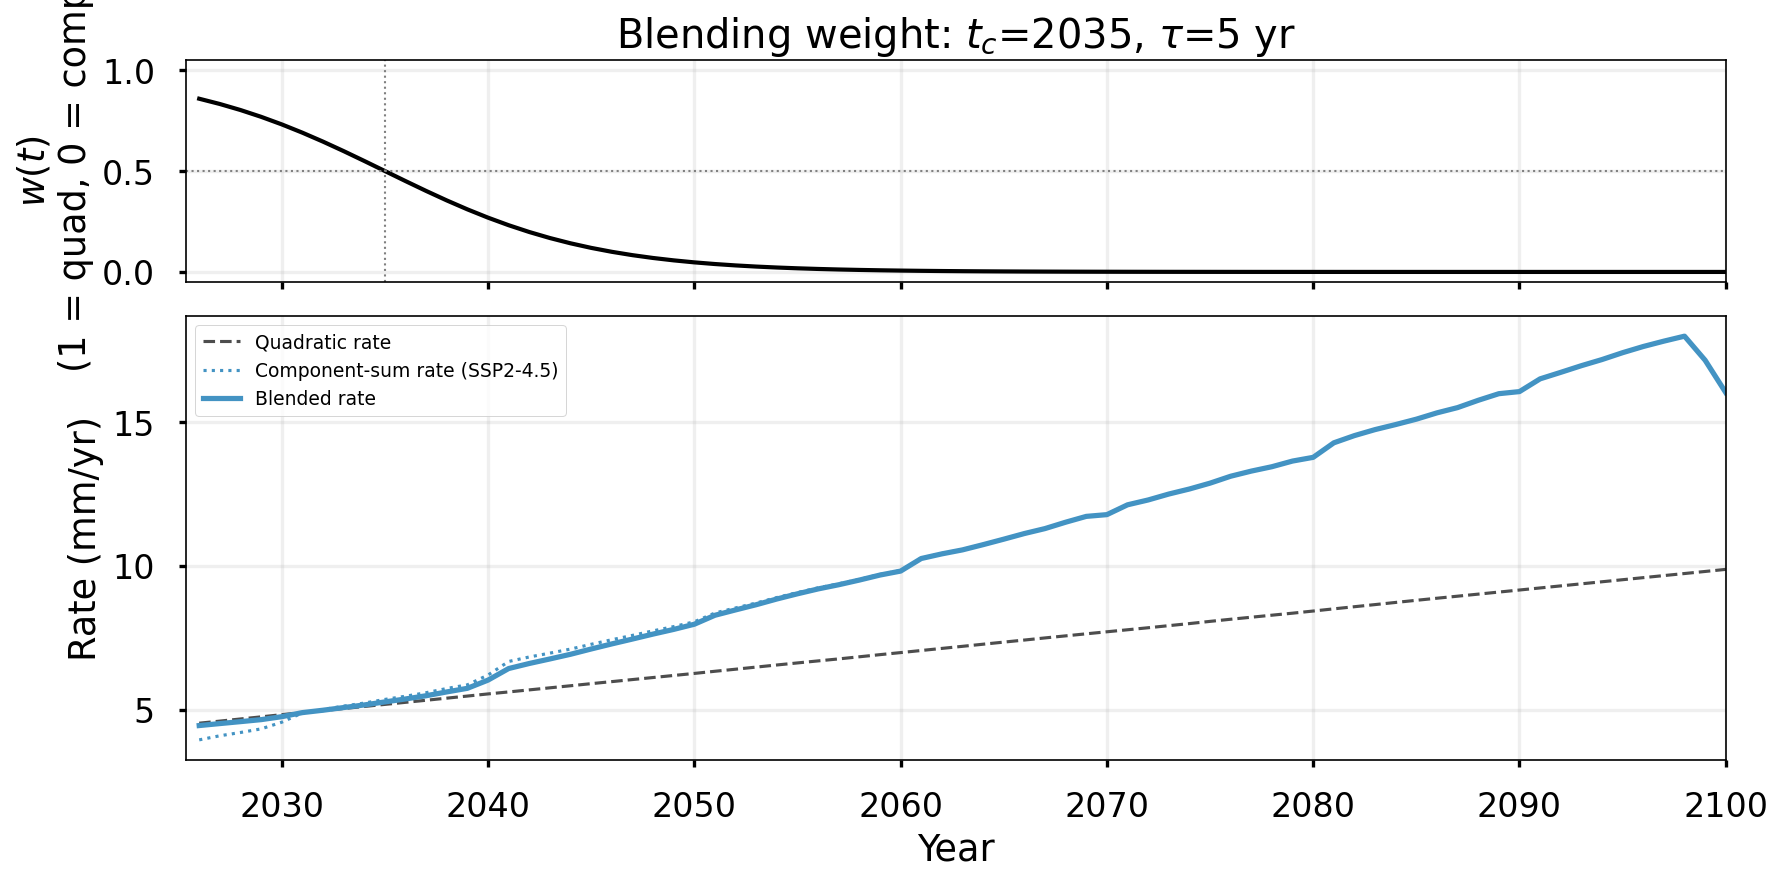
\includegraphics[width=0.48\textwidth]{component_forecast_blending_diagnostic.png}
%\caption{\textbf{Uncertainty structure of the forecast.}
%\textbf{(A)}~Exceedance probability at 2100 relative to pre-industrial
%for each SSP (colored curves), with IPCC AR6 total shown for comparison
%(grey).  The probability of exceeding 1~m is 42\% (SSP1-2.6), 58\%
%(SSP2-4.5), and 78\% (SSP3-7.0).  Averaged across policy-relevant
%pathways, $P(>1\,\mathrm{m}) = 59\%$.  The 90\% credible interval
%(143~cm for SSP2-4.5) is six times the cross-scenario median spread
%(23~cm), indicating that ice-sheet dynamics uncertainty dominates over
%emissions-pathway uncertainty.  A variance decomposition (law of total
%variance across policy SSPs) attributes 97\% of total forecast variance
%to within-scenario uncertainty (predominantly WAIS) and 3\% to
%between-scenario differences.
%\textbf{(B)}~Rate-space blending diagnostic showing the sigmoid weight
%function $w(t)$ (upper) and the blended rate for SSP2-4.5 (lower),
%transitioning from the satellite-era quadratic rate (dashed) to the
%component-sum rate (dotted) via a sigmoid centered at 2035 with width
%$\tau = 5$~yr.}
%\label{fig:uncertainty}
%\end{figure}

%% ================================================================
\subsection*{Implications}

These results have three implications for adaptation planning. First, the central estimates of sea level rise used for infrastructure decisions are too low by a factor of 1.4--1.7, with the largest discrepancy under the moderate-warming scenarios most relevant to current policy. Second, the uncertainty is wider than current assessments acknowledge, driven primarily by West Antarctic ice dynamics---a source that is not reducible by emissions mitigation on policy-relevant timescales \citep{Naughten2023}. Third, the observation that glacier mass-loss sensitivity to temperature is six times larger than embedded in process-model projections suggests that the models used to inform adaptation have not been validated against the global-scale observations now available.

The data-driven framework presented here is not a replacement for process models, which remain essential for understanding the mechanisms of ice sheet change. It is a complement: an independent, observation-anchored estimate that makes its assumptions and limitations explicit, provides an observational benchmark against which process models can be tested, and produces conditional predictive distributions that reflect what the data currently support.


%% ================================================================
%% MATERIALS AND METHODS
%% ================================================================
\section*{Materials and Methods}

\subsection*{Observational datasets}

All component models are calibrated against published observational products (Table~S1). We use:
\begin{itemize}
\item \textbf{Global mean sea level:} NASA satellite altimetry (TOPEX/Jason, 1993--present; Hamlington et~al.~\cite{Hamlington2020}), with the Frederikse et~al.~\citep{Frederikse2020} tide-gauge reconstruction (1900--2018) and Dangendorf et~al.~\citep{Dangendorf2019} reconstruction for pre-satellite validation.
\item \textbf{Ocean thermal expansion:} NOAA thermosteric sea level, 0--700\,m (1955--2025) and 0--2000\,m (2005--2025) \citep{Levitus2012}. A 14\% structural uncertainty is applied to account for the documented low bias from vertical interpolation of sparse profiles \citep{Li2022}. Depth corrections for 700--2000\,m ($0.15 \pm 0.05$~mm\,yr$^{-1}$; \cite{Levitus2012, Cheng2017}) and below 2000\,m ($0.07 \pm 0.04$~mm\,yr$^{-1}$; \cite{Purkey2010, Desbruyeres2016}) are applied cumulatively for years before full-depth data are available.
\item \textbf{Glaciers:} GlaMBIE global consensus (2000--2024; GlaMBIE~\cite{GlaMBIE2024}), combining glaciological field measurements, satellite altimetry, DEM differencing, and GRACE/GRACE-FO gravimetry across all 19 RGI regions.
\item \textbf{Greenland:} Mouginot et~al.~\citep{Mouginot2019} SMB and discharge (1972--2018), with Mankoff et~al.~\citep{Mankoff2021} (1986--2023) withheld for validation. Subsurface ocean temperature from EN4 (200--500\,m, Greenland peripheral waters; Good et~al.~\cite{Good2013}). Surface temperature from Berkeley Earth \citep{Rohde2020}.
\item \textbf{Antarctica:} IMBIE satellite-era mass balance (1992--2020; Otosaka et~al.~\cite{Otosaka2023}), partitioned by region.
\item \textbf{Terrestrial water storage:} Frederikse et~al.~\citep{Frederikse2020} reconstruction (1900--2018).
\end{itemize}

\subsection*{Component models}

\paragraph{Thermosteric.} NOAA observations with literature depth corrections (hindcast, 1950--2020) are spliced with IPCC AR6 \texttt{oceandynamics} projections (2020--2150; Fox-Kemper et~al.~\cite{Fox-Kemper2021}). The IPCC projections are generated from a two-layer energy balance model \citep{Geoffroy2013} emulated by FaIR \citep{Smith2021}, with the ensemble filtered against observed global temperature and ocean heat content. Monte Carlo samples (2000) are drawn from the IPCC 107-quantile distributions using rank-preserving uniform draws, level-matched to observations at 2020.

\paragraph{Glaciers.} The rate of glacier sea level contribution is modeled as $\dot{H}_{\mathrm{gl}} = b\,T + c$, where $T$ is GMST anomaly, calibrated against GlaMBIE using Bayesian inference with weakly informative priors. A quadratic term $a\,T^2$ is included in the prior but the posterior is centered near zero, confirming linearity over the observed range. Cumulative loss is capped at total glacier volume.

\paragraph{Greenland SMB.} Observed RACMO-derived SMB \citep{Mouginot2019} for the hindcast. Forecasts use a quadratic temperature scaling $\Delta\dot{H}_{\mathrm{smb}} = C_T\,\Delta T + C_{T^2}\,\Delta T^2$ with sensitivities drawn from the inter-RCM spread \citep{Fettweis2020, Noel2021, Glaude2024}. The linear sensitivity $C_T \sim \mathcal{N}(-200, 80^2)$~Gt\,yr$^{-1}$\,$^\circ$C$^{-1}$ of GMST encompasses the MAR, RACMO, and HIRHAM estimates.

\paragraph{Greenland discharge.} Time-delay model (Eq.~\ref{eq:greenland_dyn}) calibrated against Mouginot et~al.~\citep{Mouginot2019} discharge by weighted least squares with BIC-weighted mixing across candidate delays $\delta \in \{4, 5, 6, 7, 8\}$~yr. Ocean temperature forcing under SSP scenarios is obtained from an independently calibrated linear transfer function mapping surface temperature to EN4 subsurface temperature. Each Monte Carlo sample draws a single set of physical parameters $(\gamma, r_0, \delta, \alpha, \beta)$ and evaluates all SSP scenarios under that draw, so that inter-SSP differences isolate the effect of the emissions pathway from parameter uncertainty.

\paragraph{WAIS.} Scenario-mixture framework with three outcomes weighted by assessed probabilities: (S1)~continued present-day rates extrapolated from IMBIE, (S2)~MISI-driven acceleration (15--100~cm) with trajectory exponent and right-skewed uncertainty from grounding-line flux nonlinearity \citep{Robel2019, Schoof2007}, (S3)~MISI plus additional cliff instability. The S2 lower bound is anchored to transient-calibrated ice sheet model projections: Goldberg et~al.~\citep{Goldberg2026} constrained two independent models against observed surface elevation changes at Thwaites and found $V_{af}$ loss rates of 180--200~Gt/a by 2067 from the trunk subdomain alone, using $n = 3$ with no calving or subglacial hydrology. Integrating this trajectory to 2100, scaling to the full Thwaites catchment, and adding comparable contributions from Pine Island Glacier (33~km grounding-line retreat since 1992; Rignot et~al.~\cite{Rignot2026}), Smith/Kohler, and S1-like non-ASE basins gives a conservative total of 13~cm; the 15~cm floor accounts for the known low biases in the underlying models. Within each scenario, the 2100 endpoint is drawn from a skew-normal distribution in log-space. The log-space formulation is motivated by the multiplicative structure of the dominant uncertainties (bed geometry, basal friction, ocean thermal forcing, buttressing loss all enter as multiplicative factors on grounding-line flux $q_g \propto h_g^{\,s}$), by the positivity constraint on mass loss, and by scale invariance across scenarios spanning two orders of magnitude. The skew-normal extension captures the asymmetry arising from flux nonlinearity \citep{Robel2019}. A multiplicative rheology correction $\sim\mathcal{N}(1.28, 0.07^2)$ is applied to all scenarios \citep{Martin2026, GetraerMorlighem2025}.

\paragraph{EAIS, Peninsula.} Bayesian rate--temperature models calibrated against IMBIE regional records \citep{Otosaka2023}. EAIS is dominated by accumulation increase under warming; the Peninsula by combined SMB and discharge. EAIS is excluded from the forecast sum because the 28-year satellite record cannot reliably distinguish the accumulation response from interannual variability ($R^2 = 0.57$), making forward projections poorly constrained. The EAIS contribution is small ($-13$ to $-30$~mm at 2100, depending on scenario) and its exclusion is conservative---it would reduce the total forecast if included.

\subsection*{Budget closure diagnostic}

The residual between the component sum and NASA altimetry is distributed across components in proportion to their variances: $\mathrm{shift}_i = (\sigma_i^2 / \sum_j \sigma_j^2) \times r$, where $r$ is the total residual and $\sigma_i$ is the standard deviation of component $i$ from its Monte Carlo ensemble. This is the Bayesian posterior update under joint Gaussian assumptions, applied as a diagnostic without modifying the component posteriors. The shift-to-sigma ratio for each component tests whether the implied adjustment is within the stated uncertainty.

\subsection*{Temperature scenarios}

SSP temperature trajectories (SSP1-2.6, SSP2-4.5, SSP3-7.0, SSP5-8.5) are from IPCC AR6 assessed warming projections. Historical forcing uses Berkeley Earth monthly GMST \citep{Rohde2020}. All anomalies are relative to a 1995--2005 baseline ($\approx$2005 reference year). Forecasts extend from 2020 to 2150, with pre-2020 values from the observational record.


%% ================================================================
%% REFERENCES
%% ================================================================

\bibliographystyle{Science}
\bibliography{references}

\end{document}
